%%%%%%%%%%%%%%%%%%%%%%%%%%%%%%%%%%%%%%%%%%%%%%%%%%%%%%%%%%%%%%%%%%%%%%%%%%%%%%
%
% Main content starts here
%
%%%%%%%%%%%%%%%%%%%%%%%%%%%%%%%%%%%%%%%%%%%%%%%%%%%%%%%%%%%%%%%%%%%%%%%%%%%%%%


\chapter{Introduction}
\label{sec:introduction}



\section{Problem statement}
\section{Thesis organization and contributions}

The thesis is organized as follows:
\begin{itemize}

\item[] \emph{Chapter 2:} 
\\We further continue with the theoretical part, such as .


\item[] \emph{Chapter 3:}
\\This chapter gives an overview of the state of the art of research in 


\item[] \emph{Chapter 4:} 
\\In this chapter, we are moving into the main part of the thesis - the implementation of the described approach. Additionally, the chapter presents the results of the experiments that were made. Furthermore, we evaluate and discuss the results of the experimental part of the approach.

\item[] \emph{Chapter 5:} 
\\This chapter is devoted to applications  We also discuss possible future work and collaboration with another university group of students.

\item[] \emph{Chapter 6:} 
\\We summarize the finding of  this thesis in this chapter, review the results and discuss possible tasks for future work.

\end{itemize}


In this thesis, the following contributions are made:
\begin{enumerate}

\item We propose a similarity search approach 

\item  W....

\item  We analyze the results and performance from the experimental part of the ....

\end{enumerate}







% First Paragraph
% CORE MESSAGE OF THIS PARAGRAPH:
\todo{P1.1. What is the large scope of the problem?}
\todo{P1.2. What is the specific problem?}

% Second Paragraph
% CORE MESSAGE OF THIS PARAGRAPH:
\todo{P2.1. The second paragraph should be about what have others been doing}
\todo{P2.2. Why is the problem important? Why was this work carried out?}

% Third Paragraph
% CORE MESSAGE OF THIS PARAGRAPH:
\todo{P3.1. What have you done?}
\todo{P3.2. What is new about your work?}

% Fourth paragraph
% CORE MESSAGE OF THIS PARAGRAPH:
\todo{P4.1. What did you find out? What are the concrete results?}
\todo{P4.2. What are the implications? What does this mean for the bigger picture?}

LaTeX hints are provided in \autoref{chap:latexhints}.

\chapter{Literature Review}
In this chapter, we present the theoretical background of the basic concepts of the thesis. Moreover, we define and explain different ....


\section{Quality}
The quality is defined by several International organisations.

German Industry Standard DIN 55350 Part 11 defines, that the quality “ … comprises all characteristics and significant features of a product or an activity which relate to the satisfying of given requirements” \citet{fitzpatrick1996software}.

Another definition of quality is presented in ANSI Standard (ANSI/ASQC A3/1978), describing that the "Quality is the totality of features and characteristics of a product or a service that bears on its ability to satisfy the given needs"  \citet{fitzpatrick1996software}.

ANOTHER DEFITION comes later....

\section{Quality models}

\subsection{Quality model ISO 9126-1}
text text
e

de
de
de

\begin{table}[h!]
    \caption{Sub-characteristics of the ISO 9126-1 quality modeL.}
	\begin{tabularx}{\textwidth}{X | X }
		%\hline
	    \textbf{Quality Characteristics} & \textbf{Sub-characteristics}	
	    \\ \hline
		\\ %\hline
		Functionality
        & Suitability
        
        Accuracy
        
        Interoperability 
        
        Security
        
        Compliance			 
		
		\\ \hline
	     \\ %\hline
		Reliability    
        
        &  Maturity 
        
        Fault tolerance 
        
        Recoverability 
        
        Compliance
		
		\\ \hline
	     \\ %\hline
	    Usability       
        
        & Understandability 
        
        Learnability 
        
        Operability 
        
        Compliance
    
	    \\ \hline
	  \\ %\hline
	   Efficiency &  Time behavior 
        
        Resource behavior 
        
        Compliance    
        \\ %\hline
	    \\ \hline
	    \\ %\hline
	    
	   Maintainability	
       
       & Analyzability 
        
        Changeability 
        
        Stability 
        
        Testability 
        
        Compliance
        
	    \\ \hline
	    \\ %\hline
	    
	   Portability	
       
       & Adaptability
       
       Installability 
       
       Co-existence
       
       Replaceability 
       
       Compliance
        	   
	\end{tabularx}
	\label{tab:table1}
	
\end{table}


\subsection{Quality model ISO 25010 }


textextex

\begin{table}[h!]
    \caption{Sub-characteristics of the Quality model-ISO/IEC 25010}
	\begin{tabularx}{\textwidth}{X | X }
		%\hline
	    \textbf{Quality Characteristics} & \textbf{Sub-characteristics}	
	    \\ \hline
		\\ %\hline
		Functional Suitability
       
        & Functional completeness
        
        Functional correctness
        
        Functional appropriateness		
        
        \\ %\hline
		\\ \hline
	     \\ %\hline
		Reliability    
        
        &  Maturity 
        
        Availability
        
        Fault tolerance
        
        Recoverability
        
		\\ \hline
	     \\ %\hline
	    Performance efficiency       
        
        & Time behaviour
        
        Resource utilization
        
        Capacity
        
        
	    \\ \hline
	  \\ %\hline
	   Compatibility  
       
       &  Co-existence
       
       Interoperability   
       
     
	    \\ \hline
	    \\ %\hline
	    
	   Usability	
       
       & Appropriateness recognizability
       
       Learnability
       
       Operability
       
       User error protection
       
       User interface aesthetics

       Accessibility
       
      
	    \\ \hline
	    \\ %\hline
	    
	   Security	
       
       & Confidentiality
       
       Integrity
       
       Non-repudiation
       
       Accountability
       
       Authenticity
              
       
	    \\ \hline
	    \\ %\hline
	    
	   Maintainability	
       
       &  Modularity
       
       Reusability
       
       Analysability
       
       Modifiability
       
       Testability
     
	    \\ \hline
	    \\ %\hline
	    
	   Portability	
       
       & Adaptability
       
       Installability
       
       Replaceability
        	   
	\end{tabularx}
	\label{tab:table1}
	
\end{table}

\section{Cognitive Load Theory (CLT)}
- Relevance to Code Comprehension

\section{Theory of Program Comprehension}
- Top-Down Model: Experienced programmers use existing knowledge to understand the structure and intent of code quickly.

- Bottom-Up Model: Beginners read line-by-line, building their understanding incrementally.

- Integrated Model: A mix of both, depending on experience level and task complexity


\begin{figure} [h!]
  \centering
  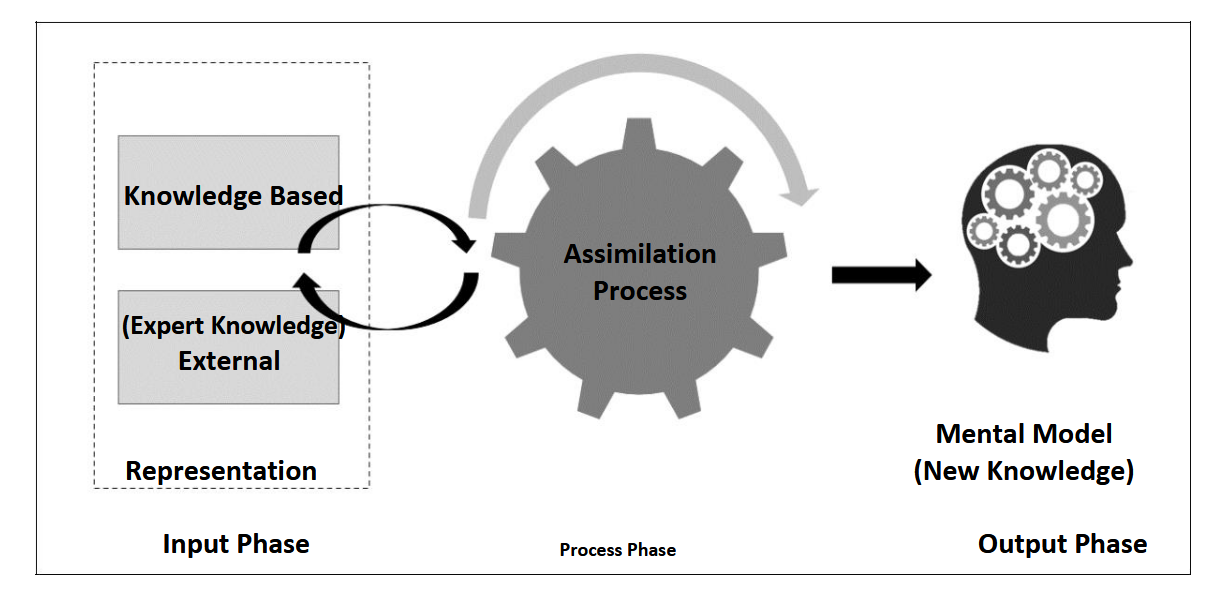
\includegraphics[width=\textwidth]{figures/program_Comprehension_Process.png}
  \caption{The Program Comprehension Process}
  \label{fig:AnhangsChor}
\end{figure}

\section{Eye Tracking}

•	Definition 


•	Background


•	Metrics


•	Why it’s relevant: Eye-tracking studies assume that where a person looks is what they are thinking about.


•	Key ideas:


o	Fixations (longer gaze duration) suggest higher cognitive processing effort.


o	Saccades (quick eye movements) indicate searching behavior (e.g., students scanning comments before reading the code).


o	Areas of Interest (AOI) refer to parts of the stimulus on which eye-tracking metrics are recorded. Examples could be chunks in the code editor, the requirements area of the IDE, or the console output. The AOI is usually defined by the researcher.


•	How to apply it:


o	Compare eye-tracking heatmaps to see if students focus more on comments before reading the code.


o	Measure how indentation influences reading patterns—does better indentation make scanning for logic structures easier?


\section{Studies using Eye Tracking}

Several studies analyze programming comprehension, using eye-tracking technology. This chapter reviews key studies, categorizing them based on their focus areas and summarizing their findings.

\subsubsection{Eye-Tracking Methodologies in Software Engineering}
The paper \citet{obaidellah2018survey} investigates the use of eye-tracking technology in computer programming research. A total of 63 relevant studies published between 1990 and June 2017 are analysed \citet{obaidellah2018survey}. The results indicate that eye-tracking technology has been applied to understand programmers' gaze pattern and cognitive processes. The studies reviewed in this paper focus on five main research fields: program comprehension and code understanding, non-code comprehension studies, debugging, requirements traceability, and collaborative programming \citet{obaidellah2018survey}.  The most frequently studied programming language is Java.  
For eye-tracking system, Tobii is the most commonly used.  Fixation duration and saccades are identified as primary metrics for analysing gaze patterns, and heatmaps are created for visual representation of the results.


\subsubsection{Variable Naming Conventions and Code Readability}

The study \citet{sharif2010eye}investigates whether different variable naming conventions (camel-case and underscore) impact code comprehension and readability.
The task of the participants was to recognize different variable names, while their eye movements were tracked and analysed from the researches. 
The findings indicate no significant difference in accuracy between the camel-case and underscore naming conventions \citet{sharif2010eye}. However, underscore identifiers were recognized 20\% faster compared to camel-case identifiers \citet{sharif2010eye}. Moreover, the data from the eye-tracking technology showed that camel-case identifiers led to longer gaze durations, more fixations, and a   higher cognitive load. Furthermore, novice programmers benefited more from the underscore variable naming conventions.   
Overall, the results indicate that underscore variable naming conventions are easier to process visually and potentially improve code readability.   


The eye-tracking study \citet{broberg2019using}investigates how different variable naming conventions impact on code readability.  
The test subjects analyzed code snippets containing variables in Single Word (SW), Single Letter (SL), Camel Case (MWCC), and Snake Case (MWSC) \citet{broberg2019using}. While explaining the code snippets, their eye movements were tracked. Researchers measured the time participants spent analysing the code and then created heatmaps to visualize their gaze patterns. Furthermore, participants provided feedback on which naming conventions they prefer. The results present no significant differences in readability using different variable naming conventions \citet{broberg2019using}. However, multi-word conventions like Snake Case and Camel Case were easier to read than Single Letter variable naming conventions \citet{broberg2019using}. The heatmaps presented that test subjects spent more time processing single-letter variables, leading to higher cognitive effort. Moreover, most participants personally found Snake Case and Camel Case easier to understand \citet{broberg2019using}. 
This study presents the role of meaningful variable naming conventions in code and how they improve code readability.   

\subsubsection{Code Transformations and Their Impact on Comprehension}
The eye-tracking study \citet{silva2023evaluating} investigates how different code transformations affect novice programmers’ code comprehension \citet{silva2023evaluating}. It focuses on Atoms of Confusion, Refactorings, and ifdef Annotations.

The findings show that confusing code snippets lead to difficulties in code comprehension and in increased fixations. Figure X presents the eye-gaze patterns for an obfuscated code snippet using the Conditional Expression atom, while Figure Y illustrates the clarified version of the same snippet \citet{silva2023evaluating}.
 
figure 1,2
\begin{figure} [h!]
  \centering
  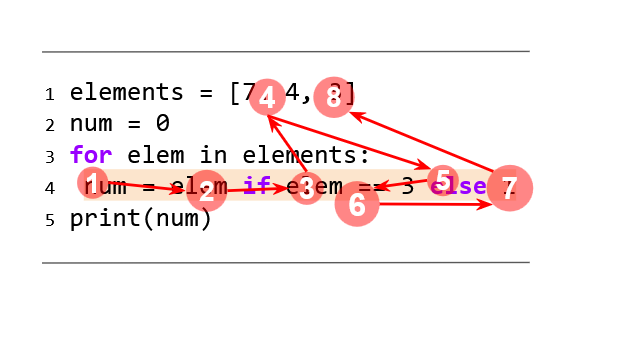
\includegraphics[scale=0.6]{figures/a.png}
  \caption{Obfuscated code snippet \citet{silva2023evaluating}}
  \label{fig:AnhangsChor}
\end{figure}

\begin{figure}
  \centering
  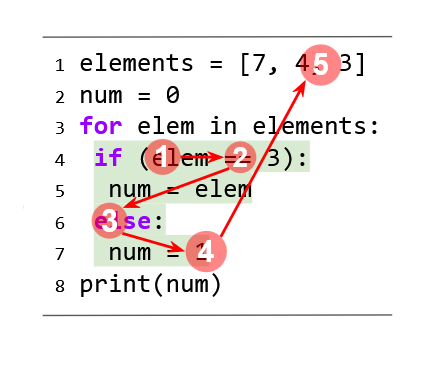
\includegraphics[scale=0.6]{figures/b.png}
  \caption{Clarified version \citet{silva2023evaluating}}
  \label{fig:AnhangsChor}
\end{figure}


\subsubsection{Program Comprehension: Iteration vs. Recursion} 
The study \citet{aroobaunderstanding} investigates how students perceive recursive and iterative programs and analyzes their cognitive processes and visual attention \citet{aroobaunderstanding}. Moreover, the study inspected whether students followed a top-down approach or bottom-up approach.
The results present that there was no significant difference between recursive and iterative programs in terms of code comprehension \citet{aroobaunderstanding}.  However, visual attention differed between iteration and recursion. 

\subsubsection{Cognitive Load and Code Complexity} 

The eye-tracking paper \citet{abbad2022estimating} investigates how to identify difficult areas of code for programmers.  Participants were given different Java code snippets and mentioned the areas of the code they found difficult \citet{abbad2022estimating}. Researchers compared the eye-tracking data with the parts marked as complicated by the participants. With the collected data, they trained machine learning models to forecast which parts of the code would challenge code comprehension \citet{abbad2022estimating}. The researches achieved more than 86\% accuracy in predicting complicated parts of code snippets. The study highlights its future usage for developing tools that can enhance code review and adaptive e-learning. 



\subsubsection{Code Structure and Indentation} 


The eye-tracking study \citet{bauer2017indentations} investigates how indentation affects comprehension. Participants analyzed Java code snippets with different levels of indentations: 0, 2, 4, and 8-space. The results presented no significant relationship between comprehension and indentation \citet{bauer2017indentations}. However, the most correct answers were given when the participants analyzed code with 4-space indentation . Furthermore, the results indicated that 8-space indentation was rated as the easiest to read level of indentation, but did not improve the accuracy of the correct answers \citet{bauer2017indentations}. Overall, eye-tracking data showed no significant differences in gaze patterns across different indentation levels, and the study highlights the need for further investigation. 



Another study \citet{yorimoto2024quantitative} investigates how indentation affects code comprehension. Students were given code tasks with different levels of indentation: 0-character, 4-character, and random indentation \citet{yorimoto2024quantitative}. The researchers measured the eye movements and cognitive load of the participants. The results showed increased confusion and cognitive load when students analyzed code with unstructured indentation \citet{yorimoto2024quantitative}. Furthermore, 4-character indentation resulted in more precise but longer focus on code areas. The study mentions that indentation had little impact on small code tasks and highlights that further investigation is needed \citet{yorimoto2024quantitative}.   



\chapter{Study Design}

\section{Methodology}

\section{Procedure}

\section{Measurements}

\section{Participants}

\chapter{Results}

\chapter{Discussion - Interpretation of Results}

\chapter{Conclusion and Outlook}
\label{sec:conclusion}
